\section{RISULTATI}
Per quanto concerne le analisi relative alle performance (in termini di f1-\textit{score}, per i motivi precedentemente discussi) di DT e RF al variare del numero di feature estratte dal processo di PCA, i risultati (riportati in Figura \ref{fig:pca-perf}) mostrano come per un numero di componenti inferiore a $10$, le performance raggiunte dai modelli siano analoghe e pessime. Il trend si inverte con il raggiungimento della componente numero $12$, dove la tendenza varia completamente, portando le performance dei modelli ad assestarsi su valori decisamente migliori; dal grafico è possibile evincere come l'aumento della dimensionalità oltre le $12$ feature garantisca un incremento delle prestazioni marginale e fortemente inconsistente.
A seguito di questa analisi, la dimensione ottimale utilizzata è pari a $12$; questo valore risulta essere un compromesso tra performance assolute e numero di feature considerate.
In particolare si può notare come gli alberi di decisione inizino a mostrare un degradamento delle performance attorno alla componente $19$, portando ad una flessione delle F1, mentre le RF tendano a migliorare leggermente le loro predizioni, presentando però continue variazioni tra una dimensione e l'altra.
\begin{figure}
	\centering
	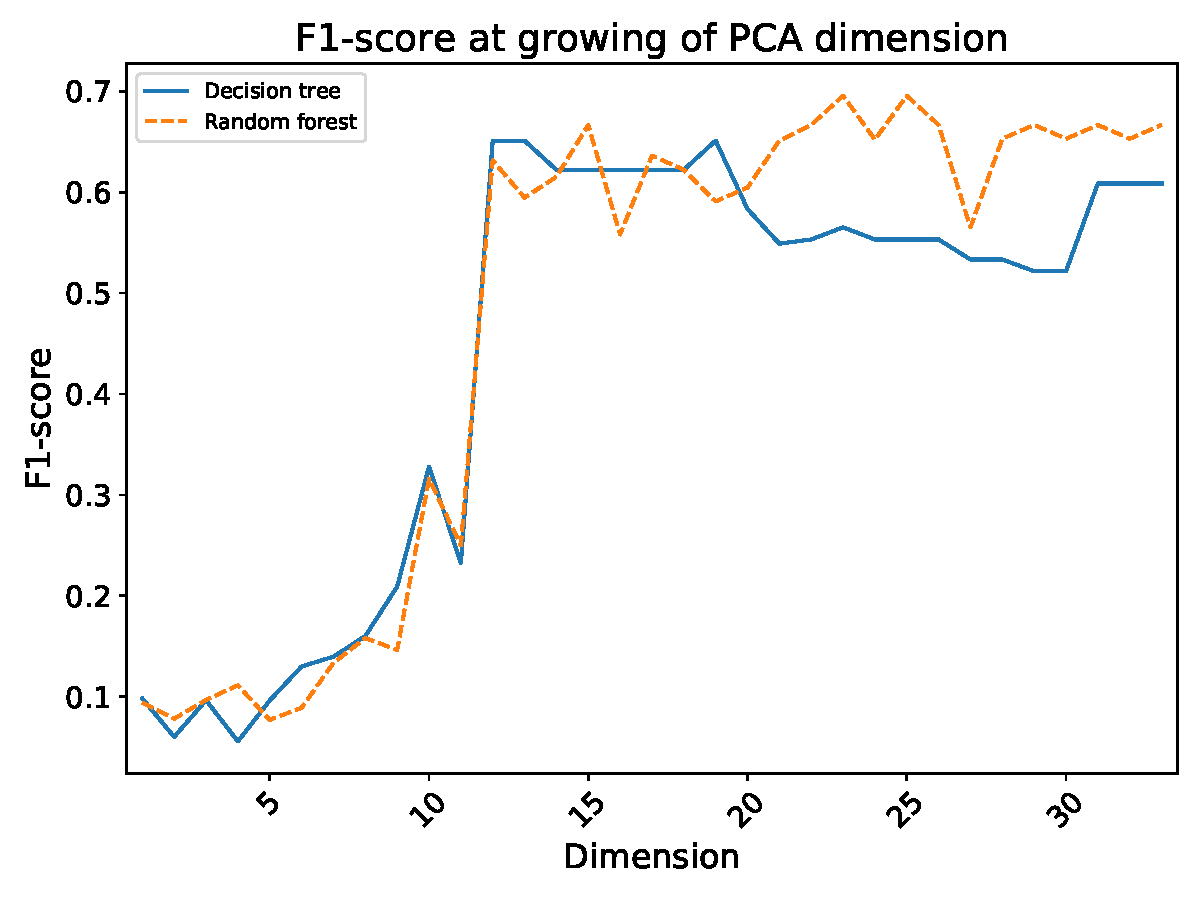
\includegraphics[width=0.9\linewidth]{images/pca-perf}
	\caption{}
	\label{fig:pca-perf}
\end{figure}

\begin{figure}
	\centering
	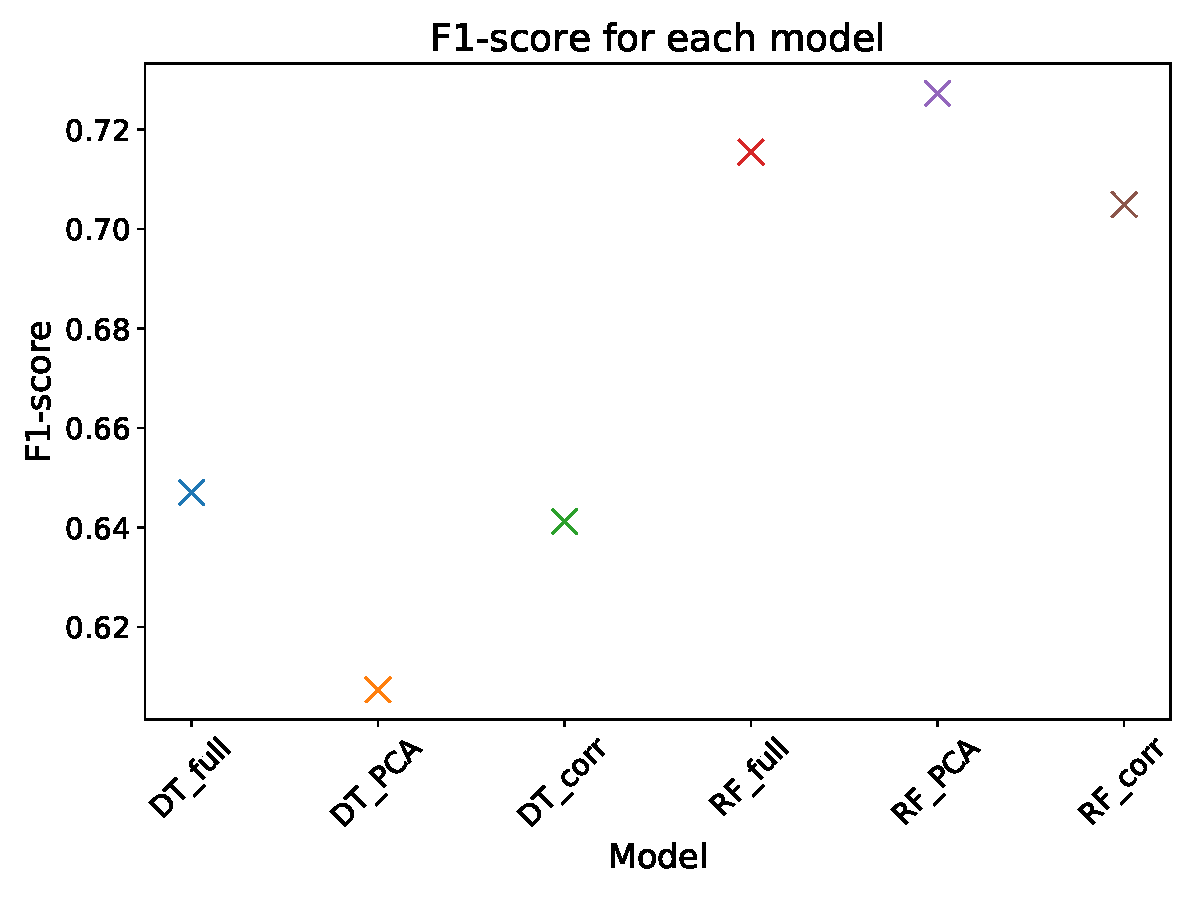
\includegraphics[width=0.8\linewidth]{images/fscore}
	\caption{}
	\label{fig:fscore}
\end{figure}

\begin{table}
\centering
\caption{Performance medie del processo di \textit{stratified 5-fold cross validation} sul dataset completo e dopo FR dei modelli analizzati.}
\label{tab:f1score}
\begin{tabular}{|c|c|c|}
	\toprule
	Modello & Tecnica da FR & F1 media \\ 
	\midrule 
	Decision Tree & / & $0.672$ \\  
	Random Forest & / & $0.673$ \\ 
	Decision Tree & Filtro correlazione & $0.607$ \\ 
	Random Forest & Filtro correlazione & $0.729$ \\ 
	Decision Tree & PCA & $0.667$ \\ 
	Random Forest & PCA & $0.619$ \\ 
	\bottomrule
\end{tabular}
\end{table}

\begin{table}
	\centering
	\caption{Performance medie del processo di \textit{stratified 5-fold cross validation} dei modelli senza considerare le feature relative ad esami strumentali effettuati sulle pazienti.}
	\label{tab:noexamsscore}
	\begin{tabular}{|c|c|}
		\toprule
		Modello & F1 media \\ 
		\midrule 
		Decision Tree & $0.21$ \\  
		Random Forest  & $0.054$ \\ 
		\bottomrule
	\end{tabular}
\end{table}

\todo[inline]{Citazione biblio è strana con o accentate grandi DP}